%# -*- coding: utf-8-unix -*-
% !TEX program = xelatex
% !TEX root = ../thesis.tex
% !TEX encoding = UTF-8 Unicode
%%==================================================
%% chapter02.tex for SJTU Master Thesis
%% based on CASthesis
%% modified by wei.jianwen@gmail.com
%% Encoding: UTF-8
%%==================================================

\chapter{Competition on two layer with different updating rules}
\label{chap:competition on two layer with different updating rules}
\section{Competition on two-layer Networks with sequential updating rule}
In this subsection, each layer consists of \textit{Barabasi-Albert(BA)} network that has $N$ nodes with attaching new nodes each with $K$ edges that are preferentially attached to existing nodes with high degree as introduced in \cite{barabasi1999}. Each node of one layer is connected with a random node on the other layer. This means each node has only $1$ external un-directed edge. Simulations are preformed on network with $N=2048$, and $K = 3$.

The simulation results are shown in Fig.~\ref{AS_2d} and Fig.~\ref{p_v_AS_3d}. Fig.~\ref{AS_2d}(a) shows that when $p > 0.2$, $0.37 < v < 0.47$, it normally tends to positive consensus. But, if $v$ is lower or larger than certain values, it doesn't make consensus.
In Fig.~\ref{AS_2d}(b), as $v$ increases, the state of networks changes continuously. But, when $p$ is very low($p \le 0.05$), it doesn't make positive consensus. On the other hands, when $p$ is large enough, it has the most positive consensus parts. When $v$ are large enough($>0.6$) and less than $1$, the state is in a coexistence part.


Fig.~\ref{p_v_AS_3d} shows the states of two layers according to all $p$s and all $v$s. The $X$-axis is the $p$ and the $Y$-axis is the $v$, and the $Z$-axis represents \textit{AS}. The closer the color is to blue, the more it has positive consensus. And the closer the color is to red, the more it has negative consensus. A light and white areas have coexistence with positive states and negative states. This chart has two areas for coexistence, when $v$ is very low or very high. When $v$ is in certain range, interconnected network can perform positive or negative consensus with different $p$ values. 

\begin{figure}[!htb]
	\centering
	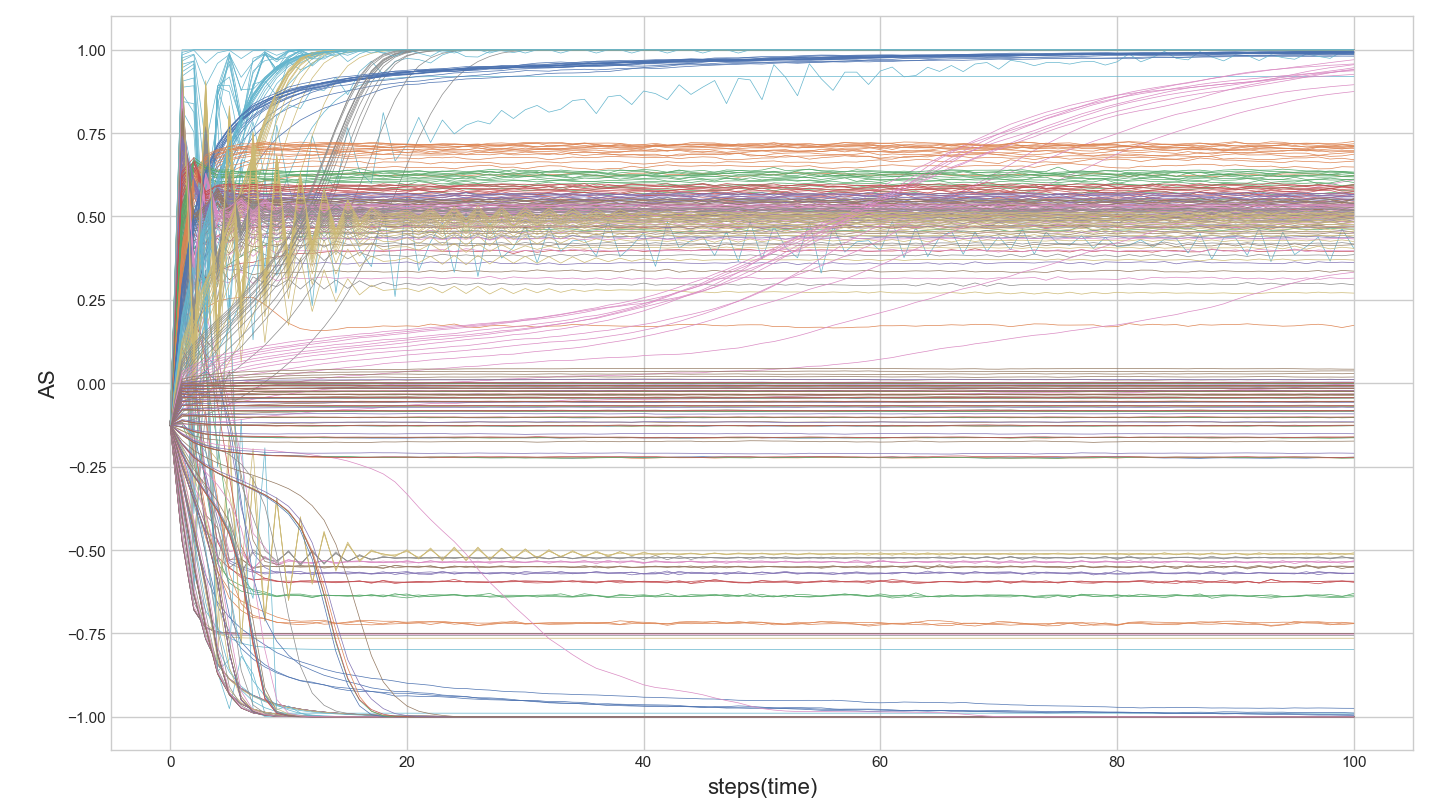
\includegraphics[width=\hsize]{figure/timeflow_AS.png}
	\caption{Two layer networks with sequential updating rule : \textit{steps-AS} changing with all $p$ and $v$}
	\label{timeflow_AS}
\end{figure}

Fig.~\ref{timeflow_AS} shows \textit{AS} value according to each step(time). As the steps are increased, the state of two-layers become stable. The closer \textit{AS} value is to $1$, the closer the state is to positive consensus. The closer \textit{AS} value is to $-1$, the closer the state is to negative consensus. \textit{AS} values between $1$ and $-1$ represents coexistence states, but it cannot be classified whether they are mixed coexistence states or separated coexistence states.
\begin{figure}[!htb]
	\centering
	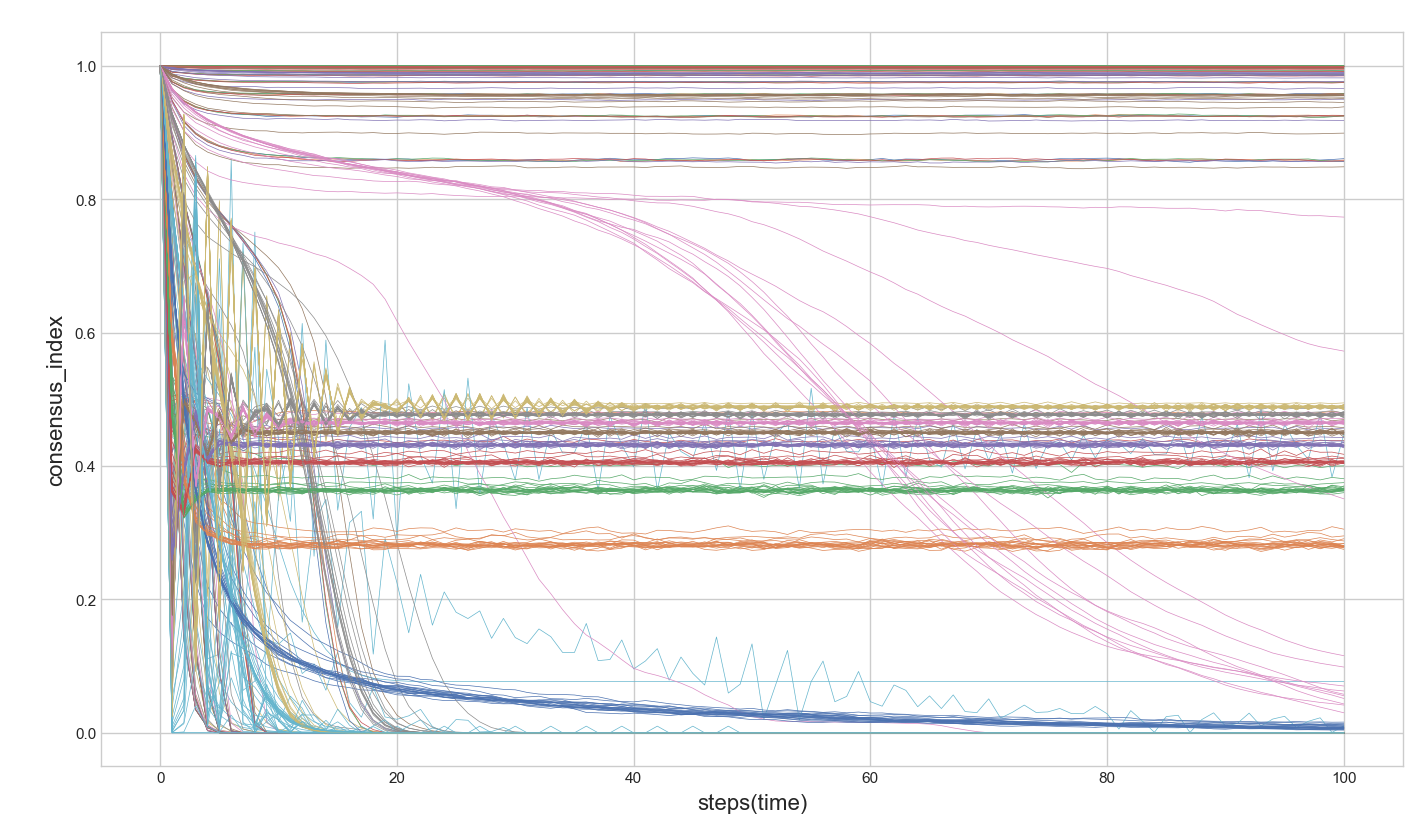
\includegraphics[width=\hsize]{figure/timeflow_CI.png}
	\caption{Two layer networks with sequential updating rule :\textit{steps-CI} changing with all $p$ and $v$}
	\label{timeflow_CI}
\end{figure}
Fig.~\ref{timeflow_CI} shows \textit{CI} value according to each step(time). With \textit{CI}, the coexistence states of two-layer can be classified into mixed coexistence states and separated coexistence states. As the \textit{CI} value is close to $0.5$, the states are close to mixed coexistence states. And, as the \textit{CI} value is close to $1$, the states are close to separated coexistence states. If the values are close to $0$, the states are close to consensus states.(Here, it is impossible to divide whether they are positive consensus or negative consensus.)           

\section{Competition on two-layer Networks with different updating rules}
When considering dynamics order on two-layer networks, there are many ways to update the state of nodes. First, order of two layer dynamics can be considered. And then order of nodes in each layer can be investigated as updating rules. In addition, order of edges in one node also can be researched. But, in layer B dynamics, order of edges in one node is always for simultaneous updating rule, because dynamics formula already considers states of all connected neighbor nodes simultaneously. To sum up, as shown in Table.\ref{table1}, 25 updating rules would be considered according to layers, nodes, and edges. 
\begin{table}[htp]
	\scriptsize
	\begin{center}
		\begin{tabular}{c|c|c|c|c}
			Order of layers                                  & \multicolumn{2}{|c|}{Layer A}                                      & Layer B                & remarks   \\ \cline{2-4}
			& Order of nodes                 & Order of edges                     & Order of nodes         &  \\ \hline
			\multirow{10}{*}{Layer A $\rightarrow$ Layer B} & \multirow{4}{*}{Sequential}    & \multirow{2}{*}{Sequential}        & Sequential             & O(o, o) $\to$ D(o) \\  \cline{4-5}  
			&                                &                                    & Simultaneous           & O(o, o) $\to$ D(s) \\  \cline{3-5}     
			&                                & \multirow{2}{*}{Simultaneous}      & Sequential             & O(o, s) $\to$ D(o) \\  \cline{4-5} 
			&                                &                                    & Simultaneous           & O(o, s) $\to$ D(s) \\  \cline{2-5} 
			& \multirow{4}{*}{Simultaneous}  & \multirow{2}{*}{Sequential}        & Sequential             & O(s, o) $\to$ D(o) \\  \cline{4-5}
			&                                &                                    & Simultaneous           & O(s, o) $\to$ D(s) \\  \cline{3-5}
			&                                & \multirow{2}{*}{Simultaneous}      & Sequential             & O(s, s) $\to$ D(o) \\  \cline{4-5}
			&                                &                                    & Simultaneous           & O(s, s) $\to$ D(s) \\  \cline{2-5}
			& \multirow{2}{*}{Random}        & \multirow{2}{*}{Random}            & Sequential             & O(r, r) $\to$ D(o) \\  \cline{4-5}
			&                                &                                    & Simultaneous           & O(r, r) $\to$ D(s) \\   \hline
			\multirow{10}{*}{Layer A $\leftarrow$ Layer B}  & \multirow{4}{*}{Sequential}    & \multirow{2}{*}{Sequential}        & Sequential             & O(o, o) $\leftarrow$ D(o) \\  \cline{4-5}  
			&                                &                                    & Simultaneous           & O(o, o) $\leftarrow$ D(s) \\  \cline{3-5}     
			&                                & \multirow{2}{*}{Simultaneous}      & Sequential             & O(o, s) $\leftarrow$ D(o) \\  \cline{4-5} 
			&                                &                                    & Simultaneous           & O(o, s) $\leftarrow$ D(s) \\  \cline{2-5} 
			& \multirow{4}{*}{Simultaneous}  & \multirow{2}{*}{Sequential}        & Sequential             & O(s, o) $\leftarrow$ D(o) \\  \cline{4-5}
			&                                &                                    & Simultaneous           & O(s, o) $\leftarrow$ D(s) \\  \cline{3-5}
			&                                & \multirow{2}{*}{Simultaneous}      & Sequential             & O(s, s) $\leftarrow$ D(o) \\  \cline{4-5}
			&                                &                                    & Simultaneous           & O(s, s) $\leftarrow$ D(s) \\  \cline{2-5}
			& \multirow{2}{*}{Random}        & \multirow{2}{*}{Random}            & Sequential             & O(r, r) $\leftarrow$ D(o) \\  \cline{4-5}
			&                                &                                    & Simultaneous           & O(r, r) $\leftarrow$ D(s) \\   \hline
			\multirow{2}{*}{Layer A $\leftrightarrow$ Layer B}& \multirow{2}{*}{Simultaneous}& Sequential                         & Simultaneous           & O(s, o) $\leftrightarrow$ D(s) \\ \cline{3-5}
			&                                & Simultaneous                       & Simultaneous           & O(s, s) $\leftrightarrow$ D(s) \\ \hline
			\multirow{3}{*}{Layer A $\Leftrightarrow$ Layer B}& \multirow{2}{*}{Sequential}  & Sequential                         & Sequential             & O(o, o) $\Leftrightarrow$ D(o) \\ \cline{3-5}
			&                                & Simultaneous                       & Sequential             & O(o, s) $\Leftrightarrow$ D(o) \\ \cline{2-5}
			& Random                         & Random                             & Random                 & O(r, r) $\Leftrightarrow$ D(r) \\ \hline
			
		\end{tabular}
	\end{center}
	\caption{25 updating rules according to order of layers, nodes, and edges}
	\label{table1}
\end{table}

In table remarks, 'O(o, o) $\to$ D(s)’ means Opinion layer(node : sequential order updating, edges : sequential order updating) $\to$ Decision Making layer(node : simultaneous updating). And 'O(o, o) $\Leftrightarrow$ D(o)’ means that one node in Opinion layer is updated, and then one node in Decision Making layer is updated, this rule is repeated until all nodes are updated.
Dynamics with 25 updating rules are simulated with parameter $p=0.4$ and $v=0.4$. Simulation results are divided by order of layers, nodes and edges. 

\subsection{Order of layers}
There exist two layers on interconnected network. And each layer have its own dynamics, such as \textit{M-Model} and \textit{AS-Model}. Two dynamics can be operated simultaneously or sequentially. If they act sequentially, dynamics of layer A can act first or dynamics of layer B can work previously. Otherwise, regardless of layers order, nodes of two layers can interact mutually. For example, one node in layer A are updated and then one node in layer B are updated until all nodes are updated.  
Considering all situations, there are 4 ways in order of two layers, \textit{Layer A $\to$ Layer B, Layer A $\leftarrow$ Layer B, Layer A $\leftrightarrow$ Layer B(simultaneous), Layer A $\Leftrightarrow$ Layer B(interaction regardless of layers)}. 
\begin{figure}[!htb]
	\centering
	\includegraphics[width=\hsize]{figure/layerorder.png}
	\caption{Simulation results according to orders of layers}
	\label{layerorder}
\end{figure}
As seen in Fig.~\ref{layerorder}, simulation results show that there is little difference between orders of layers. Consensus time and result are almost same, though dynamics order is different. Regardless of dynamics directions, when other conditions, such as order of nodes and edges are same, the dynamics results are also very similar.  

\subsection{Order of nodes}
In the simulation model, each layer has 2048 nodes, and each node has interaction with other nodes. Now, interaction order of nodes would be considered. One node can be updated after other nodes are updated. Otherwise, every node can be updated simultaneously. Simulation results would be different according to interaction order of nodes. In addition, random order between nodes is also simulated. In random order, one edge is selected randomly and updated regardless of orders between nodes and edges until all edges are considered. Interaction order of nodes have meaning related to time. If networks have short time to change states, networks follow simultaneous updating rule. However, if networks have enough time to update states, networks follow sequential updating rules. For example, discussion or conversation with enough time means sequential updating rule of nodes, and election means simultaneous updating rule of nodes. 

\begin{figure}[!htb]
	\centering
	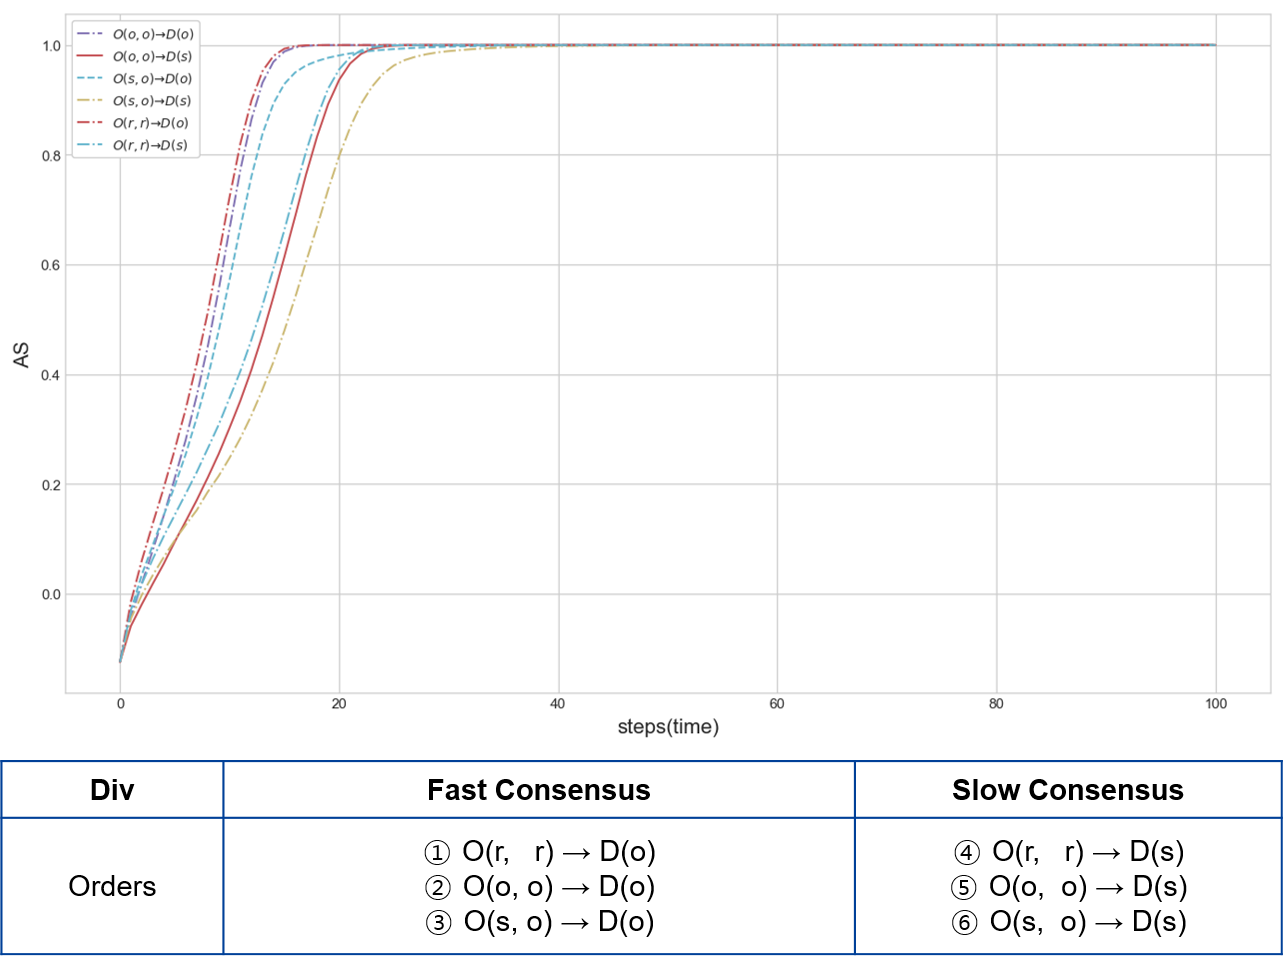
\includegraphics[width=\hsize]{figure/nodeorder.png}
	\caption{Simulation results according to orders of nodes: comparison between order of nodes under same conditions such as order of layers and edges.}
	\label{nodeorder}
\end{figure}

Simulation results shows that simultaneous interaction between nodes makes slow consensus. And, simultaneous interaction between nodes in layer B have more influence on consensus time than in layer A. Random order has similar results with sequential order and does not make different states. For quick social consensus, both opinion layer and decision making layer need sequential updating rule, such as conversation and discussion.      

\subsection{Order of edges}
Each node has some edges connected with other nodes. Simulation results can be different according to that edges are operated sequentially or simultaneously. If edges of each node work sequentially, a state of node is changed whenever each edges works. However, If edges of a node work simultaneously, a state of node has to be changed considering all connected nodes. In real world, order of edges in one node can be analyzed as characteristics of nodes. If order of edges is sequential, the node would be rash. If order of edges is simultaneous, the node would be considerate. 
\begin{figure}[!htb]
	\centering
	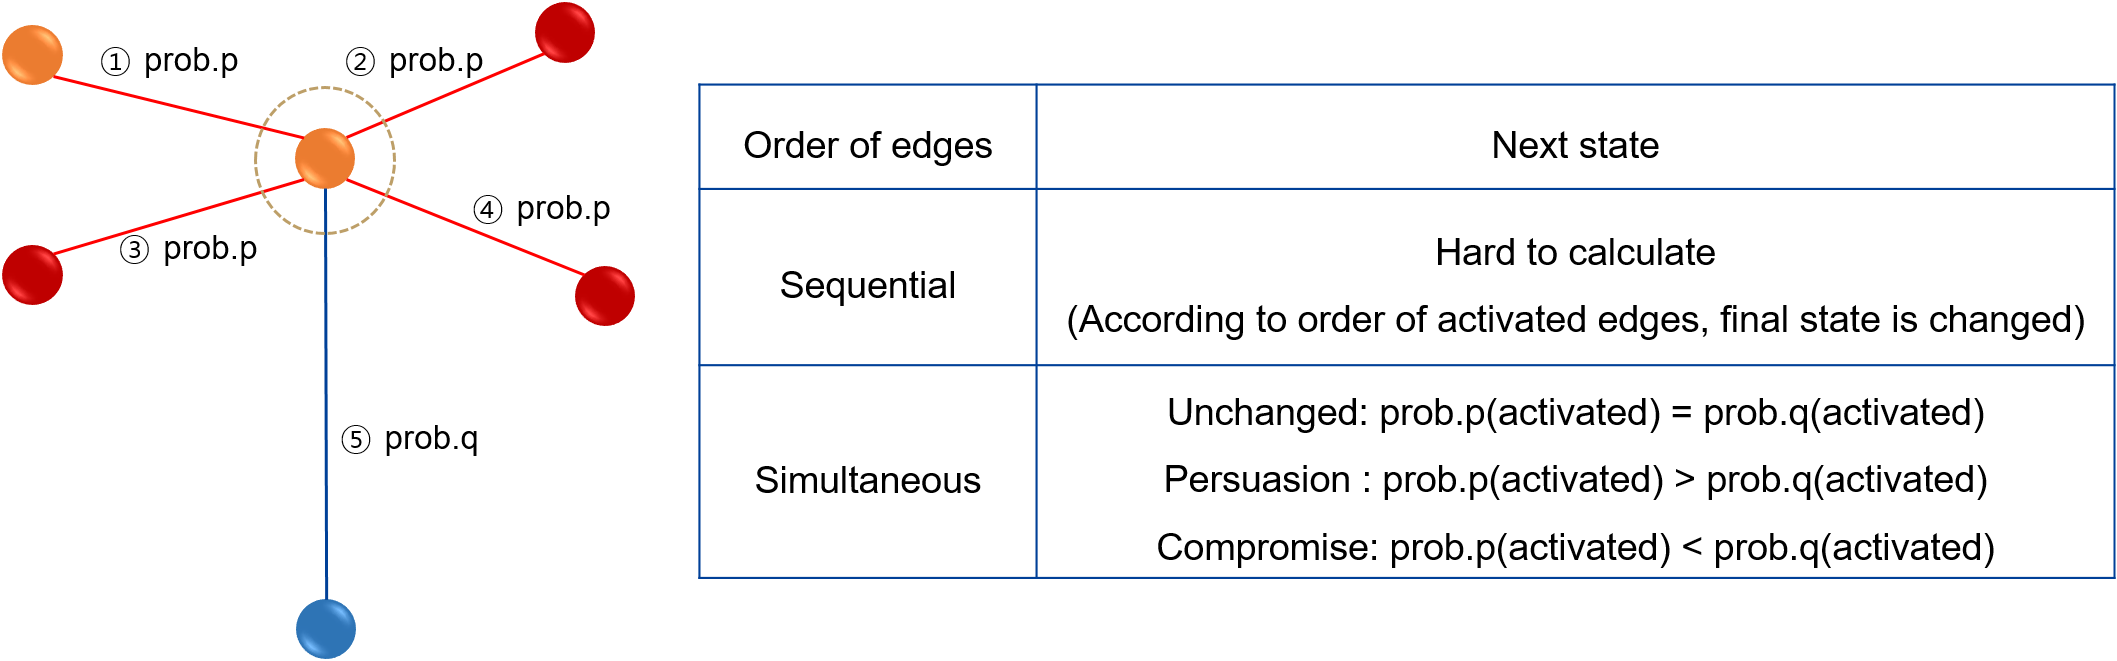
\includegraphics[width=\hsize]{figure/edgeorder_explanation.png}
	\caption{one node connected with other nodes changes its state with sequential or simultaneous order of edges}
	\label{edgeorder_explanation}
\end{figure}  
For example, considering the case that one node is connected with other nodes as shown in Fig.~\ref{edgeorder_explanation}, we can think how the state of node change. 
If the edges follow sequential updating rule, it is hard to calculate the probabilities, because the states can change according to sequential order of edges. Therefore, we can get next states of nodes by using computer simulation 

If the edges follow simultaneous updating rule, it needs some assumptions: 
\begin{enumerate}[(1)]
	\item The number of activated \textit{prob.p} is more than the number of activated \textit{prob.q}, persuasion function work. 
	\item The number of activated \textit{prob.p} is same with the number of activated \textit{prob.q}, the state would be unchanged.
	\item The number of activated \textit{prob.p} is same with the number of activated \textit{prob.q}, compromise function work.
\end{enumerate}

Through these assumptions, we can calculate probabilities of changing state in layer by considering all cases like these formula.  

\begin{equation}
\begin{array}{l}
K = \{ k \quad|\quad 0, \cdots ,{n^{ - {S_i}}}\}, \quad L = \{l \quad|\quad 0, \cdots ,{n^{{S_i}}}\},
\quad M = \{m \quad|\quad k-l\}, \\
{P_A}({S_i} \mapsto {{S'}_i}) = \begin{cases}
\mbox{unchanged}(k = l):\sum {{p^{{n^{ - {S_i}}}+m}} \cdot {{(1 - p)}^{{n^{{S_i}}}-m}} \cdot {}_{{n^{{S_{^i}}}}}{C_k} \cdot {}_{{n^{ - {S_{^i}}}}}{C_l}} \\
\mbox{persuasion}(k > l):\sum {{p^{{n^{ - {S_i}}}+m}} \cdot {{(1 - p)}^{{n^{{S_i}}}-m}} \cdot {}_{{n^{{S_{^i}}}}}{C_k} \cdot {}_{{n^{ - {S_{^i}}}}}{C_l}} \\
\mbox{compromise}(k < l):\sum {{p^{{n^{ - {S_i}}}+m}} \cdot {{(1 - p)}^{{n^{{S_i}}}-m}} \cdot {}_{{n^{{S_{^i}}}}}{C_k} \cdot {}_{{n^{ - {S_{^i}}}}}{C_l}} 
\end{cases}
\end{array}
\end{equation}

\begin{figure}[!htb]
	\centering
	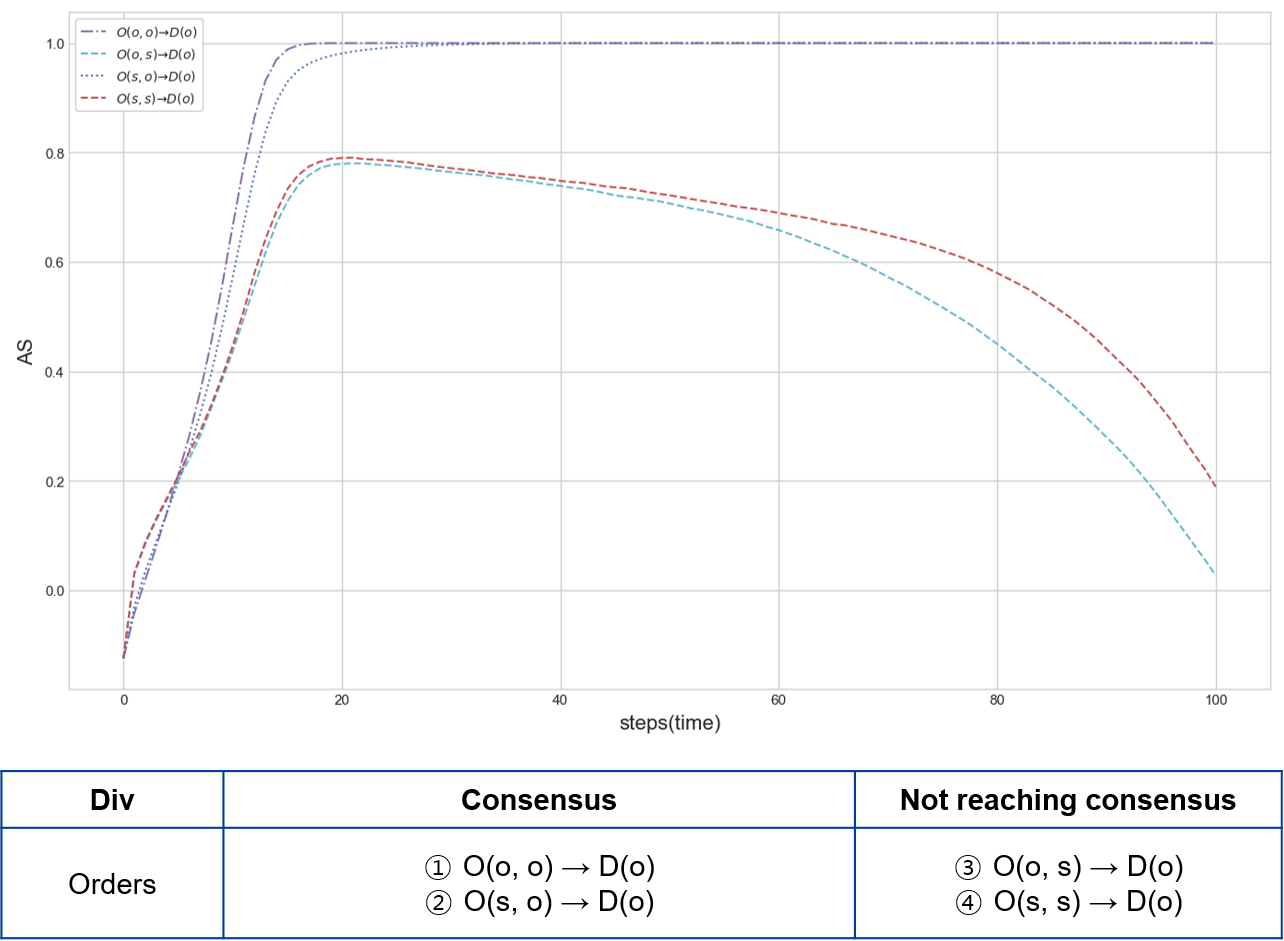
\includegraphics[width=\hsize]{figure/edgeorder.png}
	\caption{Simulation results according to orders of edges: comparison between order of edges under same conditions such as order of layers and nodes}
	\label{edgeorder}
\end{figure}
As shown in Fig.~\ref{edgeorder}, sequential updating rule of edges(rash node) makes consensus. But simultaneous updating rule of edges(considerate node) makes it hard to reach consensus. It can be analyzed that rash node is easy to be extreme and make consensus, but considerate node is very moderate and hard to reach consensus. 

\subsection{Comparison and Analysis}
It is found out that there are different simulation results according to orders of layers, nodes, and edges. To sum up all updating rules, they can be categorized into 3 parts, positive consensus, coexistence, and negative consensus as shown in Fig.~\ref{ordertotal}.  
\begin{figure}[!htb]
	\centering
	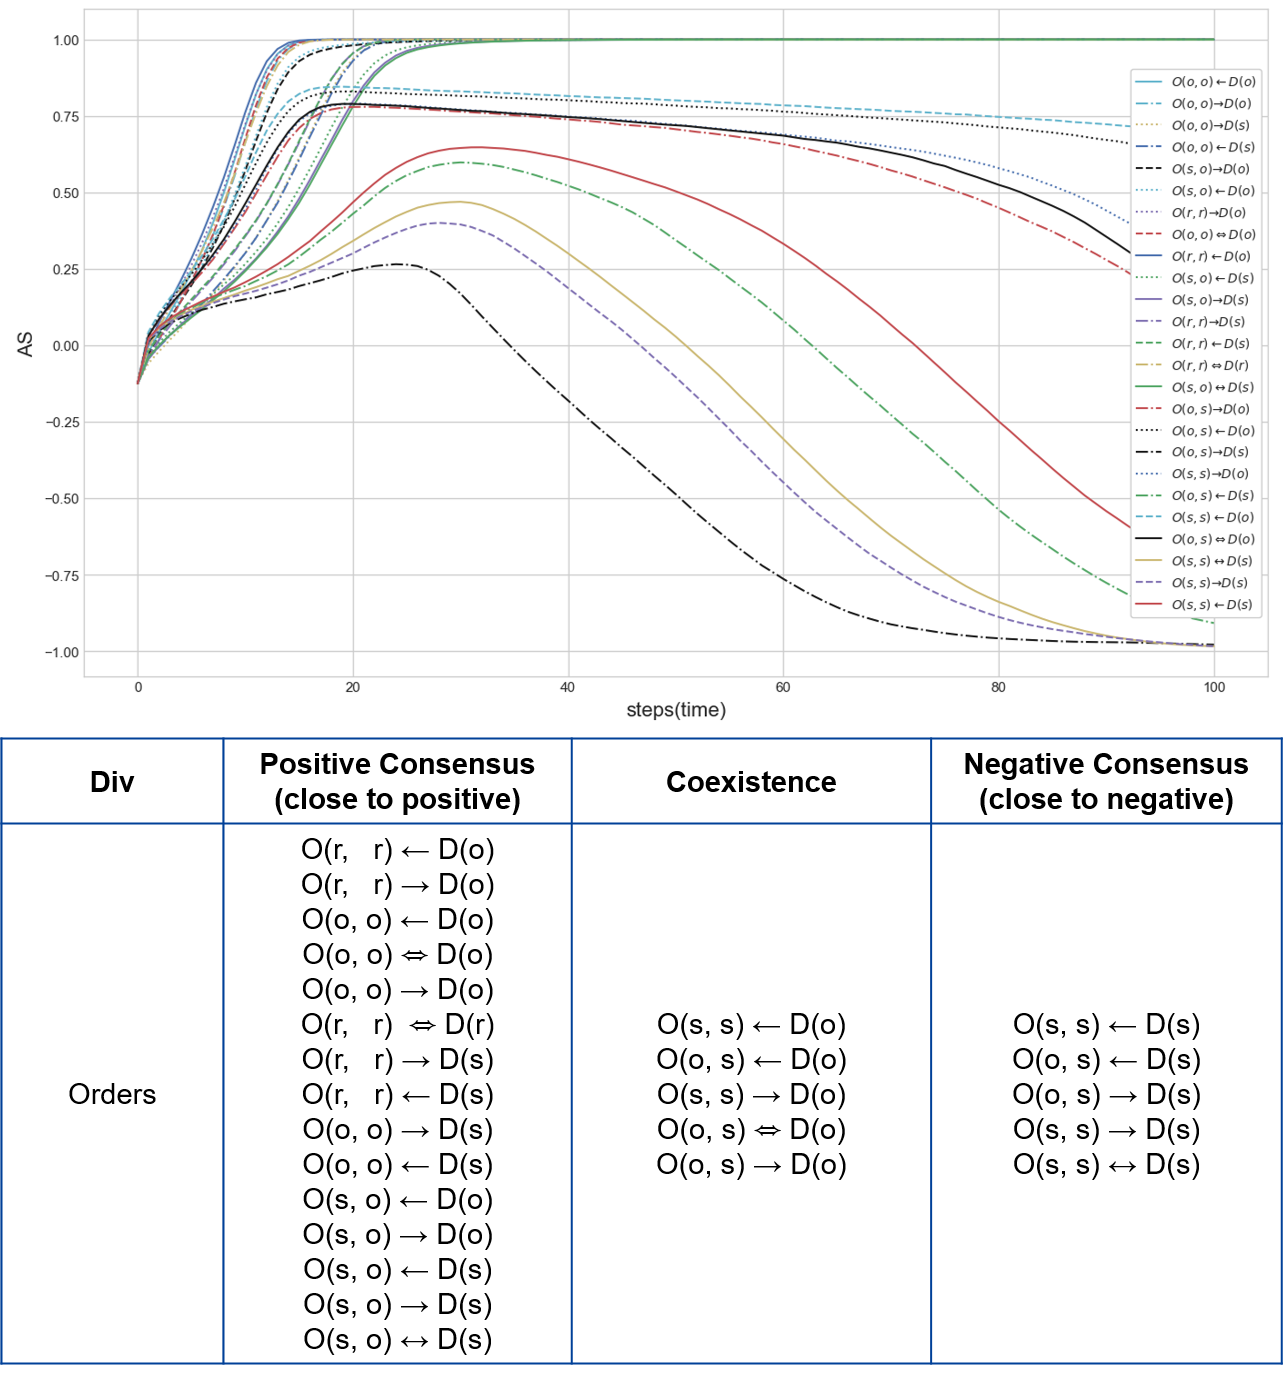
\includegraphics[width=\hsize]{figure/ordertotal.png}
	\caption{Total results of 25 updating rules with \textit{AS}}
	\label{ordertotal}
\end{figure}

To clearly classify the state of two-layers, the results can be analyzed by using \textit{CI} as shown in Fig.~\ref{ordertotal2}. There are three branch points. In the first branch point, the results are divided according to whether order of nodes in layer B is sequential or simultaneous. In the second and third branch point, the results are divided according to whether order of edges in layer A is sequential or simultaneous. As the results, there are 4 categories such as fast positive consensus, slow positive consensus, coexistence and slow negative consensus. 
\begin{figure}[!htb]
	\centering
	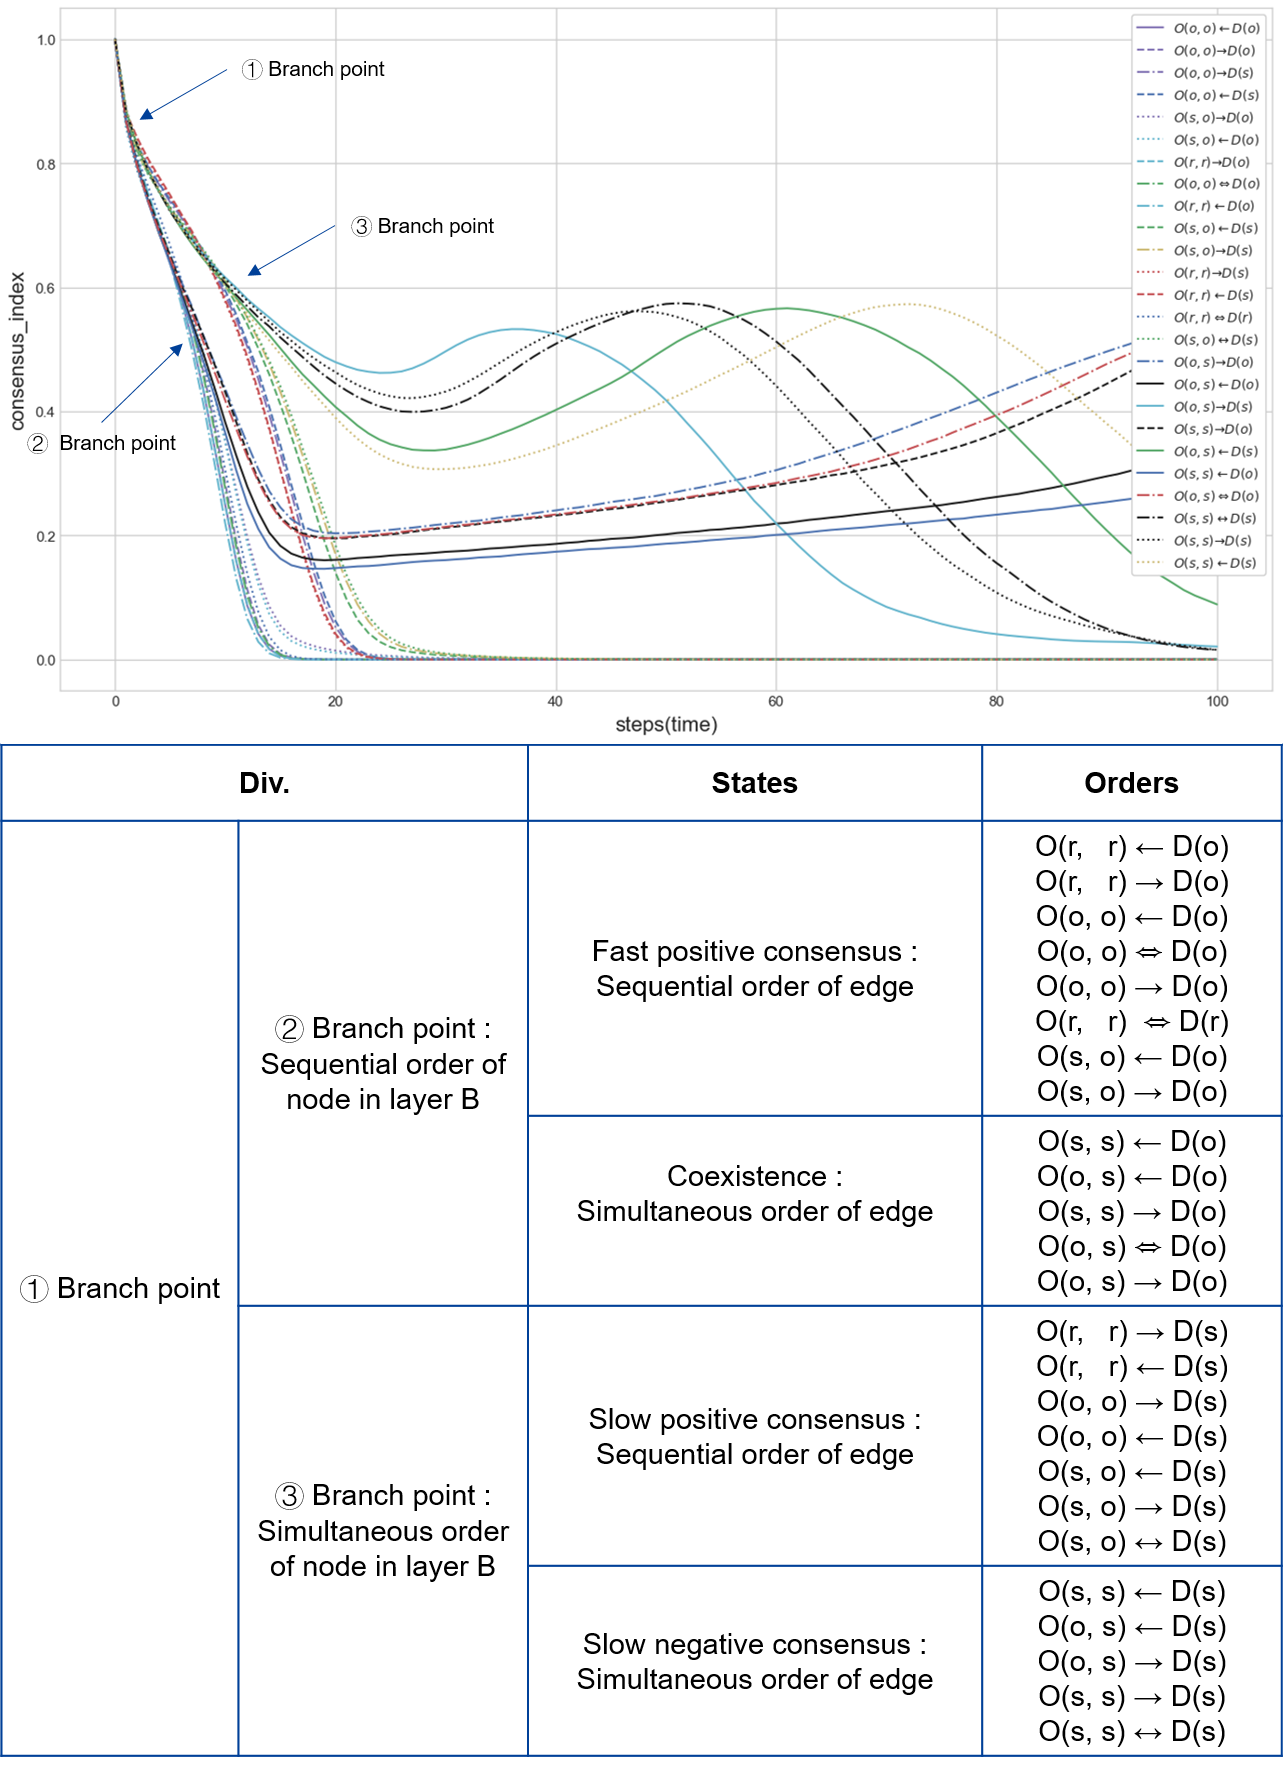
\includegraphics[width=\hsize]{figure/ordertotal2.png}
	\caption{Total results of 25 updating rules with \textit{CI}}
	\label{ordertotal2}
\end{figure}
Through these results, several important facts can be arranged. First, networks with more simultaneous updating rules make slow consensus or coexistence, sometimes make transition to opposite orientation. On the other hands, networks with more sequential updating rules make fast consensus. In other words, if opinion layer has more rash nodes, more time to have some conversation and decision making layer has more time to  discuss topics, the network have more probabilities to make consensus for opinion layer. Second, dynamics order between layers does not have an influence for network state, though there exists tiny consensus time gap. Third, order of nodes in layer B has more influence for network states than order of nodes in layer A. order of nodes in layer B makes the first branch point. But order of nodes in layer A does not make any branch point, though there exists tiny consensus time gap. Forth, order of edges in layer A is very influential so that it makes different network states. So to speak, characteristics of nodes in layer A, such as rash and considerate, affects consensus time and sometimes makes transition to coexistence or opposite orientation. 
